%==========================================
%DIF LATEXDIFF DIFFERENCE FILE
%DIF DEL /mnt/user-data/uploads/main.tex   Mon Jul 27 11:35:22 2026
%DIF ADD /mnt/user-data/outputs/main.tex   Fri Jul 31 19:57:50 2026
% SIBGRAPI 2026 -- Main Track submission (double-blind)
% Expanded version (target <= 6 pages). IEEEtran, 10pt, conference, two columns.
%==========================================
\documentclass[10pt,conference]{IEEEtran}

\usepackage{cite}
\ifCLASSINFOpdf
  \usepackage[pdftex]{graphicx}
  \graphicspath{{figs/}}
  \DeclareGraphicsExtensions{.pdf,.jpeg,.png}
\else
  \usepackage[dvips]{graphicx}
  \graphicspath{{../figs/}}
  \DeclareGraphicsExtensions{.eps}
\fi
\usepackage[cmex10]{amsmath}
\interdisplaylinepenalty=2500
\usepackage{array}
\usepackage{booktabs}
\usepackage{url}

\hyphenation{op-tical net-works semi-conduc-tor}

%-------------------------------------------------------------------------
\newif\iffinal
\finalfalse
%\finaltrue
\newcommand{\cmtid}{173} % <-- replace with the CMT submission number
%-------------------------------------------------------------------------
\iffinal\else
\usepackage[switch]{lineno}
\fi
%DIF PREAMBLE EXTENSION ADDED BY LATEXDIFF
%DIF UNDERLINE PREAMBLE %DIF PREAMBLE
\RequirePackage[normalem]{ulem} %DIF PREAMBLE
\RequirePackage{color}\definecolor{RED}{rgb}{1,0,0}\definecolor{BLUE}{rgb}{0,0,1} %DIF PREAMBLE
\providecommand{\DIFadd}[1]{{\protect\color{blue}\uwave{#1}}} %DIF PREAMBLE
\providecommand{\DIFdel}[1]{{\protect\color{red}\sout{#1}}}                      %DIF PREAMBLE
%DIF SAFE PREAMBLE %DIF PREAMBLE
\providecommand{\DIFaddbegin}{} %DIF PREAMBLE
\providecommand{\DIFaddend}{} %DIF PREAMBLE
\providecommand{\DIFdelbegin}{} %DIF PREAMBLE
\providecommand{\DIFdelend}{} %DIF PREAMBLE
\providecommand{\DIFmodbegin}{} %DIF PREAMBLE
\providecommand{\DIFmodend}{} %DIF PREAMBLE
%DIF FLOATSAFE PREAMBLE %DIF PREAMBLE
\providecommand{\DIFaddFL}[1]{\DIFadd{#1}} %DIF PREAMBLE
\providecommand{\DIFdelFL}[1]{\DIFdel{#1}} %DIF PREAMBLE
\providecommand{\DIFaddbeginFL}{} %DIF PREAMBLE
\providecommand{\DIFaddendFL}{} %DIF PREAMBLE
\providecommand{\DIFdelbeginFL}{} %DIF PREAMBLE
\providecommand{\DIFdelendFL}{} %DIF PREAMBLE
\newcommand{\DIFscaledelfig}{0.5}
%DIF HIGHLIGHTGRAPHICS PREAMBLE %DIF PREAMBLE
\RequirePackage{settobox} %DIF PREAMBLE
\RequirePackage{letltxmacro} %DIF PREAMBLE
\newsavebox{\DIFdelgraphicsbox} %DIF PREAMBLE
\newlength{\DIFdelgraphicswidth} %DIF PREAMBLE
\newlength{\DIFdelgraphicsheight} %DIF PREAMBLE
% store original definition of \includegraphics %DIF PREAMBLE
\LetLtxMacro{\DIFOincludegraphics}{\includegraphics} %DIF PREAMBLE
\newcommand{\DIFaddincludegraphics}[2][]{{\color{blue}\fbox{\DIFOincludegraphics[#1]{#2}}}} %DIF PREAMBLE
\newcommand{\DIFdelincludegraphics}[2][]{% %DIF PREAMBLE
\sbox{\DIFdelgraphicsbox}{\DIFOincludegraphics[#1]{#2}}% %DIF PREAMBLE
\settoboxwidth{\DIFdelgraphicswidth}{\DIFdelgraphicsbox} %DIF PREAMBLE
\settoboxtotalheight{\DIFdelgraphicsheight}{\DIFdelgraphicsbox} %DIF PREAMBLE
\scalebox{\DIFscaledelfig}{% %DIF PREAMBLE
\parbox[b]{\DIFdelgraphicswidth}{\usebox{\DIFdelgraphicsbox}\\[-\baselineskip] \rule{\DIFdelgraphicswidth}{0em}}\llap{\resizebox{\DIFdelgraphicswidth}{\DIFdelgraphicsheight}{% %DIF PREAMBLE
\setlength{\unitlength}{\DIFdelgraphicswidth}% %DIF PREAMBLE
\begin{picture}(1,1)% %DIF PREAMBLE
\thicklines\linethickness{2pt} %DIF PREAMBLE
{\color[rgb]{1,0,0}\put(0,0){\framebox(1,1){}}}% %DIF PREAMBLE
{\color[rgb]{1,0,0}\put(0,0){\line( 1,1){1}}}% %DIF PREAMBLE
{\color[rgb]{1,0,0}\put(0,1){\line(1,-1){1}}}% %DIF PREAMBLE
\end{picture}% %DIF PREAMBLE
}\hspace*{3pt}}} %DIF PREAMBLE
} %DIF PREAMBLE
\LetLtxMacro{\DIFOaddbegin}{\DIFaddbegin} %DIF PREAMBLE
\LetLtxMacro{\DIFOaddend}{\DIFaddend} %DIF PREAMBLE
\LetLtxMacro{\DIFOdelbegin}{\DIFdelbegin} %DIF PREAMBLE
\LetLtxMacro{\DIFOdelend}{\DIFdelend} %DIF PREAMBLE
\DeclareRobustCommand{\DIFaddbegin}{\DIFOaddbegin \let\includegraphics\DIFaddincludegraphics} %DIF PREAMBLE
\DeclareRobustCommand{\DIFaddend}{\DIFOaddend \let\includegraphics\DIFOincludegraphics} %DIF PREAMBLE
\DeclareRobustCommand{\DIFdelbegin}{\DIFOdelbegin \let\includegraphics\DIFdelincludegraphics} %DIF PREAMBLE
\DeclareRobustCommand{\DIFdelend}{\DIFOaddend \let\includegraphics\DIFOincludegraphics} %DIF PREAMBLE
\LetLtxMacro{\DIFOaddbeginFL}{\DIFaddbeginFL} %DIF PREAMBLE
\LetLtxMacro{\DIFOaddendFL}{\DIFaddendFL} %DIF PREAMBLE
\LetLtxMacro{\DIFOdelbeginFL}{\DIFdelbeginFL} %DIF PREAMBLE
\LetLtxMacro{\DIFOdelendFL}{\DIFdelendFL} %DIF PREAMBLE
\DeclareRobustCommand{\DIFaddbeginFL}{\DIFOaddbeginFL \let\includegraphics\DIFaddincludegraphics} %DIF PREAMBLE
\DeclareRobustCommand{\DIFaddendFL}{\DIFOaddendFL \let\includegraphics\DIFOincludegraphics} %DIF PREAMBLE
\DeclareRobustCommand{\DIFdelbeginFL}{\DIFOdelbeginFL \let\includegraphics\DIFdelincludegraphics} %DIF PREAMBLE
\DeclareRobustCommand{\DIFdelendFL}{\DIFOaddendFL \let\includegraphics\DIFOincludegraphics} %DIF PREAMBLE
%DIF COLORLISTINGS PREAMBLE %DIF PREAMBLE
\RequirePackage{listings} %DIF PREAMBLE
\RequirePackage{color} %DIF PREAMBLE
\lstdefinelanguage{DIFcode}{ %DIF PREAMBLE
%DIF DIFCODE_UNDERLINE %DIF PREAMBLE
  moredelim=[il][\color{red}\sout]{\%DIF\ <\ }, %DIF PREAMBLE
  moredelim=[il][\color{blue}\uwave]{\%DIF\ >\ } %DIF PREAMBLE
} %DIF PREAMBLE
\lstdefinestyle{DIFverbatimstyle}{ %DIF PREAMBLE
	language=DIFcode, %DIF PREAMBLE
	basicstyle=\ttfamily, %DIF PREAMBLE
	columns=fullflexible, %DIF PREAMBLE
	keepspaces=true %DIF PREAMBLE
} %DIF PREAMBLE
\lstnewenvironment{DIFverbatim}{\lstset{style=DIFverbatimstyle}}{} %DIF PREAMBLE
\lstnewenvironment{DIFverbatim*}{\lstset{style=DIFverbatimstyle,showspaces=true}}{} %DIF PREAMBLE
%DIF END PREAMBLE EXTENSION ADDED BY LATEXDIFF

\begin{document}

\title{Visual Similarity Is Not Enough: Domain-Adapted Synthetic Data \\ for Maritime Vessel Detection}

\iffinal
\author{\IEEEauthorblockN{Anonymous Authors}
\IEEEauthorblockA{Anonymous Institution}}
\else
  \author{SIBGRAPI Paper ID: \cmtid \\ }
  \linenumbers
\fi

\maketitle

\begin{abstract}
Operational maritime surveillance systems require large annotated datasets, yet
coastal and port-monitoring imagery is scarce and difficult to annotate. Large
public ship datasets seem an obvious remedy, but we show that using one
($\sim$28{,}000 images) for pre-training causes \emph{negative transfer},
reducing mAP50 by 4.15 points relative to a COCO-pretrained baseline, because of
a structural domain gap in scale (ships occupy $\sim$\DIFdelbegin \DIFdel{54}\DIFdelend \DIFaddbegin \DIFadd{39}\DIFaddend \% versus $\sim$0.1\% of the
image), object density, and capture conditions; curating the public images by
\DIFaddbegin \DIFadd{global, whole-image }\DIFaddend visual similarity does not prevent this, and an epoch
ablation shows the degradation grows monotonically with exposure. We propose \emph{in-place
synthetic composition}: vessel crops segmented with a foundation segmentation
model from public images are resized and placed at the positions and scales of
real vessels in operational scenes. Balanced joint training of real and
synthetic images improves mAP50 by 1.00 point and Recall by 2.2 points over the
COCO baseline \DIFdelbegin \DIFdel{, with the largest relative gain }\DIFdelend \DIFaddbegin \DIFadd{(seed-paired $p<0.05$), with gains across all object sizes and the
largest point estimate }\DIFaddend in small-object recall. An ablation
shows that anchoring crops to real vessel positions is not the main driver:
sea-aware random placement performs comparably. A volume-matched control confirms that the in-domain mAP50 gain stems from synthetic diversity rather than training volume, and that this effect is even more pronounced under zero-shot evaluation on an independent maritime dataset.
\end{abstract}

\IEEEpeerreviewmaketitle

\section{Introduction}
Maritime vessel detection underpins coastal surveillance, search and rescue,
port safety, and traffic monitoring. Detectors of the YOLO family
\cite{redmon2016you,jocher2023ultralytics} achieve strong results on standard
benchmarks, but operational deployment faces a fundamental obstacle: operational
datasets are small, access-restricted, and captured under conditions that differ
markedly from public maritime imagery.

The operational dataset studied here, CITRA-3D-Real, was collected under an
institutional maritime surveillance programme using fixed coastal cameras
overlooking a bay. It contains only 2{,}081 images with 7{,}003 bounding boxes,
vessels appear as small, distant objects (71.6\% are ``small'' by COCO
standards), and scenes are crowded (mean 3.37 objects per image). A large public
dataset of ship photographs, InaTechShips \cite{teixeira2025inatechships}
($\sim$28{,}000 images from a ship-spotting community), is an attractive source
of extra training data. An intuitive hypothesis is that pre-training on these
images---especially those selected for visual similarity to the operational
domain via CLIP embeddings \cite{radford2021learning}---would improve detection after
fine-tuning.

We show that this intuition does not hold in the studied setting, and we use the
experimental progression to localise \emph{why}. Our findings are threefold.
(i)~\textbf{Negative transfer from structural, not semantic, mismatch.}
Pre-training on InaTechShips, whether curated by CLIP similarity or randomly
selected, degrades mAP50 by 3.5--4.2 points relative to COCO-pretrained weights;
the equivalence of curated and random subsets indicates that global visual
similarity is an insufficient proxy for transferability.
(ii)~\textbf{Structural realignment dissects the cause.} Holding the source
vessel content fixed and progressively realigning it to the target
structure---sequential pre-training on scale-, density-, and context-matched
composites, then balanced joint training---moves the outcome from $-4.15$ (A)
through $-1.31$ (A$'$ seq) to $+1.00$ (A$'$ joint), localising the failure to
object-level structure and showing that positive transfer additionally requires
the joint regime. (iii)~\textbf{Spatial anchoring is data hygiene.} An ablation
shows that placing synthetic crops at exact real-vessel positions is not the
source of the gain. Finally, a zero-shot evaluation on an independent dataset
confirms the directional effects on an unseen domain.

\section{Related Work}

\textbf{Copy-paste augmentation.} Copy-paste compositing~\cite{ghiasi2021simple} creates training images by pasting object instances onto backgrounds, and has proven effective for detection and segmentation under limited data. In the maritime domain it has been applied with synthetic or metadata-guided placement: Poseidon~\cite{ruizponce2023poseidon} generates synthetic training images using metadata to constrain placement, and Ribeiro et al.~\cite{ribeiro2022synthetic} use automatically annotated synthetic videos to train real-time ship segmentation. Recent variants combine controlled copy-paste with adaptive blending for maritime scenarios using DETR variant\cite{nemati2025rtdetr}. A common limitation is that placement decisions are either heuristic (sample uniformly within a plausible region) or driven by external metadata; neither guarantees alignment with the operational distribution of vessel positions. Unlike these methods, we anchor synthetic vessels to the positions of real annotated vessels in operational scenes, which removes arbitrary placement decisions and, by construction, reproduces the operational scale and density. Our spatial-anchoring ablation (Section \ref{subsec:inplace}) further shows that the joint balanced regime is robust to placement choice within the sea region, isolating the contribution of crop diversity from that of exact anchoring.

\textbf{Transfer and negative transfer.} Initialising detectors from large datasets such as COCO~\cite{lin2014microsoft} is standard, but domain-specific pre-training does not always help: source knowledge can degrade target performance under distributional mismatch~\cite{zhang2023negative}, and sequential fine-tuning can overwrite previously learned features~\cite{mccloskey1989catastrophic}. \DIFdelbegin \DIFdel{Comprehensive surveys of forgettingin deep learning}\DIFdelend \DIFaddbegin \DIFadd{Surveys of forgetting}\DIFaddend ~\cite{yang2024forgetting} distinguish harmful \DIFdelbegin \DIFdel{forgetting—which degrades performance—}\DIFdelend from beneficial forgetting\DIFdelbegin \DIFdel{that can aid generalisation. Transfer effectiveness depends on }\DIFdelend \DIFaddbegin \DIFadd{; transfer effectiveness tracks }\DIFaddend the similarity of the underlying data distributions rather than visual appearance~\cite{cui2018large}\DIFaddbegin \DIFadd{, }\DIFaddend and task affinity \DIFdelbegin \DIFdel{does not follow intuitive expectations}\DIFdelend \DIFaddbegin \DIFadd{defies intuition}\DIFaddend ~\cite{zamir2018taskonomy}: visually similar datasets can \DIFdelbegin \DIFdel{produce very different transfer outcomes }\DIFdelend \DIFaddbegin \DIFadd{transfer very differently }\DIFaddend when their object-level structure differs. Domain-adaptation methods explicitly align features across domains~\cite{chen2018domain}. We provide empirical evidence for this principle in maritime detection: datasets that look alike (both contain ships) but differ distributionally (scale, density, context) produce negative rather than positive transfer. A volume-matched control further shows that the contribution of training volume to the transfer outcome is itself domain-dependent: neutral within-domain but actively detrimental under domain shift (Sections \ref{subsec:inplace}, \ref{subsec:zeroshot}).

\textbf{Maritime detection and small-object benchmarks.} Most public maritime datasets consist of close-range photographs in which vessels are prominent~\cite{shao2018seaships,teixeira2025inatechships}, creating a mismatch with operational scenarios where ships are small and distant. Recent works in maritime detection have specifically targeted small-vessel scenarios: S3Det~\cite{li2024s3det} couples Normalized Wasserstein Distance with Feedback Cut\&Paste augmentation, and attention-enhanced architectures address long-distance vessel detection from ship-bridge cameras~\cite{zhang2025longdistance}. Lightweight detectors have been developed for visual wave gliders~\cite{ding2025waveglider}, and Ship\_YOLO~\cite{li2025shipyolo} reports general ship detection across visible-light, infrared, and SAR modalities.
 Across these works, however, the relationship between large public ship datasets and small-distant operational settings is rarely interrogated directly. The scale discrepancy between \DIFdelbegin \DIFdel{$\sim 54\%$ }\DIFdelend \DIFaddbegin \DIFadd{$\sim 39\%$ median }\DIFaddend image area in ship-spotting photographs and $\sim 0.1\%$ in operational surveillance is the central domain gap studied here, and—as our experiments show—its effect cannot be eliminated by visual-similarity curation alone.

 \textbf{Cross-domain evaluation}. Object-detection benchmarks typically report results on i.i.d. test splits, but operational deployment increasingly demands cross-domain evaluation~\cite{oza2023uda}. Maritime work in this direction includes evaluations across MaSTr1325 and SMD with weak annotations~\cite{bovcon2022slr}. Our work adds zero-shot evaluation on an independent maritime dataset (SMD on-shore subset) as part of the experimental design, not as post-hoc validation, allowing us to test whether the in-domain effects—negative transfer of public pre-training and benefit of domain-adapted composition—are properties of the approach or artefacts of a specific test set.

\section{Datasets and Method}

\subsection{Datasets and the domain gap}
\textbf{CITRA-3D-Real} (operational) provides 2{,}081 images
(1{,}348/332/401 train/val/test) at $1920\times1080$, spanning clear, overcast,
and hazy conditions, with all vessels collapsed to a single \emph{vessel} class.
%
\textbf{InaTechShips} \cite{teixeira2025inatechships} (public) consists of
close-range ship photographs in which a single vessel dominates the frame. We use
a CLIP-curated subset (cosine similarity $\ge 0.60$ to CITRA-3D-Real,
$\sim$27.8k images) and a random control of matched size. Because both datasets depict ships, this threshold is permissive: about 99\% of InaTechShips images exceed it, so global CLIP embeddings deem almost the entire public set similar to the operational domain. The curated and random subsets thus largely coincide, and their equivalent negative transfer (Table~\ref{tab:main}) shows that even near-maximal global similarity fails to predict transferability; \DIFaddbegin \DIFadd{Section~\ref{subsec:negativetransfer} shows that }\DIFaddend a stricter top-$k$ \DIFdelbegin \DIFdel{similarity criterion is left to future work}\DIFdelend \DIFaddbegin \DIFadd{criterion would not change this}\DIFaddend . Table~\ref{tab:gap}
contrasts the two datasets along the three axes that define the gap: objects are
roughly \DIFdelbegin \DIFdel{$500\times$ }\DIFdelend \DIFaddbegin \DIFadd{$400\times$ }\DIFaddend smaller and far denser in the operational domain (Fig.~\ref{fig:scale}).
%
\textbf{Cross-domain evaluation set.} For the zero-shot generalisation analysis (Section \ref{subsec:zeroshot}), we use the visible on-shore subset of the Singapore Maritime Dataset (SMD) \cite{prasad2017video}, filtering for fixed-camera coastal footage, collapsing annotations to a single \emph{vessel} class, and re-splitting by source video to preclude leakage. Frames are temporally subsampled, yielding 914 images from 36 videos. No SMD images are used in training; the dataset is used exclusively to evaluate trained models in the zero-shot regime.

\begin{table}[!t]
\DIFdelbeginFL %DIFDELCMD < \renewcommand{\arraystretch}{1.15}
%DIFDELCMD < %%%
\DIFdelendFL \DIFaddbeginFL \renewcommand{\arraystretch}{1.05}
\DIFaddendFL \caption{The domain gap between the operational and public datasets. \DIFaddbeginFL \DIFaddFL{COCO size
categories computed on normalised areas over a $640\times640$ canvas, matching
the network input resolution.}\DIFaddendFL }
\label{tab:gap}
\centering
\footnotesize
\setlength{\tabcolsep}{4pt}
\begin{tabular}{@{}lcc@{}}
\toprule
Property & CITRA-3D-Real & InaTechShips \\
\midrule
Median vessel area (\% of image) & $0.10$ & \DIFdelbeginFL \DIFdelFL{$\sim 54$ }\DIFdelendFL \DIFaddbeginFL \DIFaddFL{$39$ }\DIFaddendFL \\
Objects per image (mean)         & $3.37$ & \DIFdelbeginFL \DIFdelFL{$\sim 1$ }\DIFdelendFL \DIFaddbeginFL \DIFaddFL{$1.0$ }\DIFaddendFL \\
Small objects (COCO, \%)         & $71.6$ & $\sim 0$ \\
Capture style                    & operational & close-range \\
                                 & surveillance & photography \\
\bottomrule
\end{tabular}
\end{table}

\begin{figure*}[!t]
\centering
\DIFdelbeginFL %DIFDELCMD < 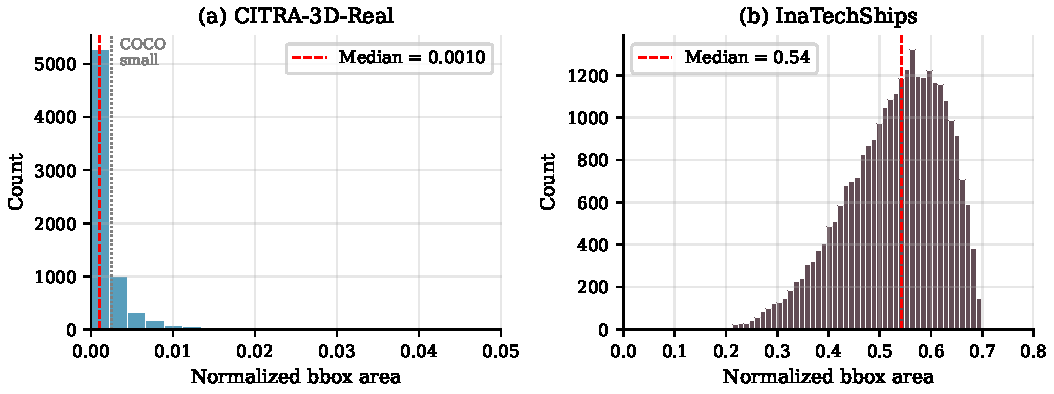
\includegraphics[width=0.8\textwidth]{fig3_scale_distribution}
%DIFDELCMD < %%%
\DIFdelendFL \DIFaddbeginFL 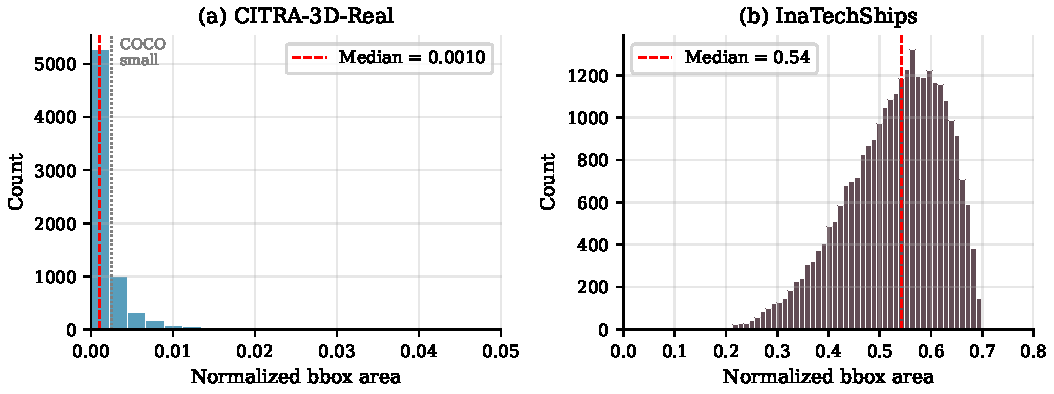
\includegraphics[width=0.66\textwidth]{fig3_scale_distribution}
\DIFaddendFL \caption{Normalised bounding-box area distributions. Operational vessels
(CITRA-3D-Real, median $0.10\%$ of the image) are far smaller than public ship
photographs (InaTechShips \DIFaddbeginFL \DIFaddFL{pre-training set}\DIFaddendFL , median \DIFdelbeginFL \DIFdelFL{$\sim$54\%}\DIFdelendFL \DIFaddbeginFL \DIFaddFL{$39\%$}\DIFaddendFL ), which is the core of
the domain gap.}
\label{fig:scale}
\end{figure*}


\subsection{In-place synthetic composition}
For each curated public image, a foundation segmentation model
\cite{kirillov2023segment} extracts the vessel as an RGBA crop using the dataset
bounding box as prompt (85.7\% usable yield after a quality filter). For each
operational training image, every annotated vessel is replaced by a randomly
selected crop, resized to the exact bounding box and alpha-blended into the scene
(Fig.~\ref{fig:pipeline}). Labels are inherited from the operational annotations,
so the synthetic images preserve the spatial distribution, density, and visual
context of the operational domain while introducing vessel appearance diversity
from the public dataset. We generate 13 variations per operational image
\DIFaddbegin \DIFadd{(1}{\DIFadd{,}}\DIFadd{348 real training images $\rightarrow$ 17}{\DIFadd{,}}\DIFadd{524 synthetic images). In the
balanced joint regime the real training set is repeated $13\times$ to match, so
one A$'$~joint epoch contains 35}{\DIFadd{,}}\DIFadd{048 images (17}{\DIFadd{,}}\DIFadd{524 real + 17}{\DIFadd{,}}\DIFadd{524
synthetic, 50/50 by construction)}\DIFaddend . The train/val/test split is fixed before
generation, and no test image, annotation, or background is used in any
training stage.

\DIFaddbegin \DIFadd{For the A$'$~joint-rand ablation, real vessels are first removed by fast-marching
inpainting }\cite{telea2004image} \DIFadd{(radius 3\,px), and crops are placed by
rejection sampling at uniformly distributed positions within a sea region
defined by an adaptive horizon (the top of the highest real bounding box), a
floor at 35\% of the image height, and an HSV-based refinement that excludes
vertical obstacles. Crop sizes are drawn from the empirical width--height
distribution of all real boxes, independently of vertical position---perspective
is deliberately }\emph{\DIFadd{not}} \DIFadd{modelled---and the number of objects per image is
preserved. Placements require at least 75\% of the box inside the sea region and
pairwise IoU below 0.2.
}

\DIFaddend \begin{figure*}[!t]
\centering
\DIFdelbeginFL %DIFDELCMD < 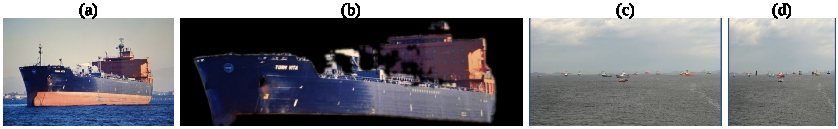
\includegraphics[width=0.8\textwidth]{fig_composition_process}
%DIFDELCMD < %%%
\DIFdelendFL \DIFaddbeginFL 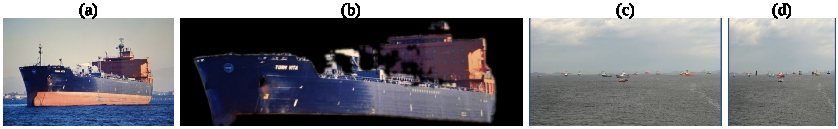
\includegraphics[width=\textwidth]{fig_composition_process}
\DIFaddendFL \caption{In-place synthetic composition. \DIFdelbeginFL \DIFdelFL{A vessel is segmented from }\DIFdelendFL \DIFaddbeginFL \DIFaddFL{(}\DIFaddendFL a\DIFdelbeginFL \DIFdelFL{public ship
}\DIFdelendFL \DIFaddbeginFL \DIFaddFL{)~Public source }\DIFaddendFL image
\DIFdelbeginFL \DIFdelFL{, }\DIFdelendFL \DIFaddbeginFL \DIFaddFL{(InaTechShips); (b)~SAM-segmented crop; (c)~operational scene (CITRA-3D-Real);
(d)~synthetic image: the crop is }\DIFaddendFL resized \DIFdelbeginFL \DIFdelFL{, }\DIFdelendFL and composited at the position \DIFaddbeginFL \DIFaddFL{and
scale }\DIFaddendFL of \DIFdelbeginFL \DIFdelFL{a }\DIFdelendFL \DIFaddbeginFL \DIFaddFL{each }\DIFaddendFL real vessel\DIFdelbeginFL \DIFdelFL{in an operational
scene}\DIFdelendFL , \DIFdelbeginFL \DIFdelFL{yielding a synthetic image with inherited labels}\DIFdelendFL \DIFaddbeginFL \DIFaddFL{inheriting its label}\DIFaddendFL .}
\label{fig:pipeline}
\end{figure*}

\subsection{Experimental setup}
All experiments use YOLOv11m \cite{jocher2023ultralytics} for single-class detection,
initialised from COCO unless stated otherwise, image size 640, AdamW, 300
fine-tuning epochs, three seeds (42, 123, 2024); results are mean $\pm$ standard
deviation on the CITRA-3D-Real test set\DIFdelbegin \DIFdel{. }\DIFdelend \DIFaddbegin \DIFadd{, and significance is assessed with
two-sided seed-paired $t$-tests (seeds matched across
arms).}\footnote{\DIFadd{With $n{=}3$ seeds an exact sign-permutation test cannot attain
$p<0.25$; the paired $t$-test is therefore the appropriate small-sample choice.}} \DIFaddend We compare: \textbf{B1} (random
initialisation), \textbf{B2} (COCO baseline), \textbf{A} (COCO $\rightarrow$
curated InaTechShips $\rightarrow$ fine-tune), \textbf{B} (COCO $\rightarrow$
random InaTechShips $\rightarrow$ fine-tune), \textbf{A$'$ joint} (COCO \DIFdelbegin \DIFdel{,
}\DIFdelend \DIFaddbegin \DIFadd{$\rightarrow$
}\DIFaddend real+synthetic combined 50/50 in a single run), and \textbf{A$'$ joint-rand} (as
A$'$ joint, but synthetic crops placed at uniformly sampled positions within the
sea region instead of at real-vessel positions). We also report two intermediate
synthetic regimes: \textbf{A$'$ seq.} (\DIFdelbegin \DIFdel{sequential }\DIFdelend \DIFaddbegin \DIFadd{a two-stage pipeline: 100 epochs of
}\DIFaddend pre-training on \DIFdelbegin \DIFdel{synthetic data}\DIFdelend \DIFaddbegin \DIFadd{the synthetic set, then 300 epochs of fine-tuning on real
CITRA-3D-Real only---unlike A$'$~joint, the two data sources are never mixed}\DIFaddend )
and \textbf{A$'$ frozen} (\DIFdelbegin \DIFdel{synthetic pre-training with a frozen backbone }\DIFdelend \DIFaddbegin \DIFadd{as A$'$ seq., with the backbone frozen during the
synthetic stage}\DIFaddend ). A volume-matched control (B2-long) oversamples the real CITRA-3D-Real images by 13$\times$ (matching the number of training images per epoch of A$'$joint) without any synthetic data, isolating the effect of training volume from synthetic diversity. Code and
configurations are available at an anonymised
repository.\footnote{\url{https://anonymous.4open.science/r/maritime-synthetic-detection-5582}}

\section{Experiments and Results}

\subsection{Negative transfer}
\DIFaddbegin \label{subsec:negativetransfer}
\DIFaddend 

Table~\ref{tab:main} reports the main results, and Fig.~\ref{fig:comparison} visualises them. COCO pre-training (B2) clearly
improves over random initialisation (B1). Pre-training on InaTechShips
\emph{hurts}: both the curated (A) and random (B) subsets fall about four points
below B2 \DIFaddbegin \DIFadd{in every seed (both $p\le0.005$)}\DIFaddend , and their near-equivalence (\DIFdelbegin \DIFdel{within one standard deviation}\DIFdelend \DIFaddbegin \DIFadd{$p=0.71$}\DIFaddend ) indicates
that the degradation stems from structural domain incompatibility rather than the
selection strategy---global CLIP similarity does not capture the scale, density,
and capture-context mismatch. \DIFaddbegin \DIFadd{A stricter threshold would not help: recomputing
the curation score for all 27}{\DIFadd{,}}\DIFadd{796 curated images and profiling similarity
deciles shows the ranking to be nearly orthogonal to the structural axes
(Spearman $\rho=-0.15$ against vessel area). Even the top-5\% most similar
images have a median vessel area of 29\% (versus 0.1\% operationally), and the
public set's object density is constant at one vessel per image (versus 3.4), so
no global-similarity threshold can close the structural gap.
}\DIFaddend 

To distinguish recoverable overfitting from fundamental incompatibility, we vary
the number of pre-training epochs on the curated subset (Fig.~\ref{fig:epochs}).
Degradation is \emph{monotonic}: even ten epochs of exposure already reduce mAP50
\DIFaddbegin \DIFadd{($0.821\pm0.004$, below the baseline in all three seeds)}\DIFaddend , and at one hundred
epochs performance approaches the random-initialisation level \DIFaddbegin \DIFadd{($0.794\pm0.005$;
10 vs.\ 100 epochs seed-paired $p=0.028$)}\DIFaddend .
This suggests that extended pre-training on the public domain progressively
overwrites the generic COCO features that are useful for the operational domain,
consistent with a forgetting-like mechanism \cite{mccloskey1989catastrophic}.

\begin{table*}[!t]
\DIFdelbeginFL %DIFDELCMD < \renewcommand{\arraystretch}{1.15}
%DIFDELCMD < %%%
\DIFdelendFL \DIFaddbeginFL \renewcommand{\arraystretch}{1.05}
\DIFaddendFL \caption{Results on the CITRA-3D-Real test set (mean $\pm$ std \DIFdelbeginFL \DIFdelFL{, }\DIFdelendFL \DIFaddbeginFL \DIFaddFL{over }\DIFaddendFL 3 seeds\DIFaddbeginFL \DIFaddFL{,
in \%}\DIFaddendFL ). $\Delta$ is the mAP50 difference versus B2 in \DIFaddbeginFL \DIFaddFL{percentage }\DIFaddendFL points.}
\label{tab:main}
\centering
\footnotesize
\setlength{\tabcolsep}{4pt}
\begin{tabular}{@{}lcccc@{}}
\toprule
Method & mAP50 & mAP50-95 & Recall & $\Delta$ \\
\midrule
A$'$ joint-rand (ablation) & \DIFdelbeginFL \DIFdelFL{$0.8457 \pm 0.0058$ }\DIFdelendFL \DIFaddbeginFL \DIFaddFL{$84.57 \pm 0.58$ }\DIFaddendFL & \DIFdelbeginFL \DIFdelFL{$0.5208 \pm 0.0024$ }\DIFdelendFL \DIFaddbeginFL \DIFaddFL{$52.08 \pm 0.24$ }\DIFaddendFL & \DIFdelbeginFL \DIFdelFL{$0.804$ }\DIFdelendFL \DIFaddbeginFL \DIFaddFL{$80.4$ }\DIFaddendFL & $+1.06$ \\
A$'$ joint (proposed)      & \DIFdelbeginFL \DIFdelFL{$0.8451 \pm 0.0033$ }\DIFdelendFL \DIFaddbeginFL \DIFaddFL{$84.51 \pm 0.33$ }\DIFaddendFL & \DIFdelbeginFL \DIFdelFL{$0.5206 \pm 0.0017$ }\DIFdelendFL \DIFaddbeginFL \DIFaddFL{$52.06 \pm 0.17$ }\DIFaddendFL & \DIFdelbeginFL \DIFdelFL{$0.805$ }\DIFdelendFL \DIFaddbeginFL \DIFaddFL{$80.5$ }\DIFaddendFL & $+1.00$ \\
A$'$ frozen                & \DIFdelbeginFL \DIFdelFL{$0.8342 \pm 0.0039$ }\DIFdelendFL \DIFaddbeginFL \DIFaddFL{$83.42 \pm 0.39$ }\DIFaddendFL & \DIFdelbeginFL \DIFdelFL{$0.5074 \pm 0.0035$ }\DIFdelendFL \DIFaddbeginFL \DIFaddFL{$50.74 \pm 0.35$ }\DIFaddendFL & \DIFdelbeginFL \DIFdelFL{$0.774$ }\DIFdelendFL \DIFaddbeginFL \DIFaddFL{$77.4$ }\DIFaddendFL & $-0.09$ \\
B2 (COCO, reference)       & \DIFdelbeginFL \DIFdelFL{$0.8351 \pm 0.0020$ }\DIFdelendFL \DIFaddbeginFL \DIFaddFL{$83.51 \pm 0.20$ }\DIFaddendFL & \DIFdelbeginFL \DIFdelFL{$0.5055 \pm 0.0022$ }\DIFdelendFL \DIFaddbeginFL \DIFaddFL{$50.55 \pm 0.22$ }\DIFaddendFL & \DIFdelbeginFL \DIFdelFL{$0.783$ }\DIFdelendFL \DIFaddbeginFL \DIFaddFL{$78.3$ }\DIFaddendFL & ref \\
B2-long (volume control)   & \DIFdelbeginFL \DIFdelFL{$0.8351 \pm 0.0025$ }\DIFdelendFL \DIFaddbeginFL \DIFaddFL{$83.51 \pm 0.25$ }\DIFaddendFL & \DIFdelbeginFL \DIFdelFL{$0.5100 \pm 0.0038$ }\DIFdelendFL \DIFaddbeginFL \DIFaddFL{$51.00 \pm 0.38$ }\DIFaddendFL & \DIFdelbeginFL \DIFdelFL{$0.796$ }\DIFdelendFL \DIFaddbeginFL \DIFaddFL{$79.6$ }\DIFaddendFL & $+0.00$ \\
A$'$ seq.                  & \DIFdelbeginFL \DIFdelFL{$0.8221 \pm 0.0085$ }\DIFdelendFL \DIFaddbeginFL \DIFaddFL{$82.21 \pm 0.85$ }\DIFaddendFL & \DIFdelbeginFL \DIFdelFL{$0.4933 \pm 0.0059$ }\DIFdelendFL \DIFaddbeginFL \DIFaddFL{$49.33 \pm 0.59$ }\DIFaddendFL & \DIFdelbeginFL \DIFdelFL{$0.769$ }\DIFdelendFL \DIFaddbeginFL \DIFaddFL{$76.9$ }\DIFaddendFL & $-1.31$ \\
B1 (random init)           & \DIFdelbeginFL \DIFdelFL{$0.8008 \pm 0.0061$ }\DIFdelendFL \DIFaddbeginFL \DIFaddFL{$80.08 \pm 0.61$ }\DIFaddendFL & \DIFdelbeginFL \DIFdelFL{$0.4742 \pm 0.0006$ }\DIFdelendFL \DIFaddbeginFL \DIFaddFL{$47.42 \pm 0.06$ }\DIFaddendFL & \DIFdelbeginFL \DIFdelFL{$0.750$ }\DIFdelendFL \DIFaddbeginFL \DIFaddFL{$75.0$ }\DIFaddendFL & $-3.43$ \\
B (InaTech random)         & \DIFdelbeginFL \DIFdelFL{$0.7945 \pm 0.0046$ }\DIFdelendFL \DIFaddbeginFL \DIFaddFL{$79.45 \pm 0.46$ }\DIFaddendFL & \DIFdelbeginFL \DIFdelFL{$0.4728 \pm 0.0045$ }\DIFdelendFL \DIFaddbeginFL \DIFaddFL{$47.28 \pm 0.45$ }\DIFaddendFL & \DIFdelbeginFL \DIFdelFL{$0.734$ }\DIFdelendFL \DIFaddbeginFL \DIFaddFL{$73.4$ }\DIFaddendFL & $-4.06$ \\
A (InaTech curated)        & \DIFdelbeginFL \DIFdelFL{$0.7936 \pm 0.0049$ }\DIFdelendFL \DIFaddbeginFL \DIFaddFL{$79.36 \pm 0.49$ }\DIFaddendFL & \DIFdelbeginFL \DIFdelFL{$0.4692 \pm 0.0017$ }\DIFdelendFL \DIFaddbeginFL \DIFaddFL{$46.92 \pm 0.17$ }\DIFaddendFL & \DIFdelbeginFL \DIFdelFL{$0.735$ }\DIFdelendFL \DIFaddbeginFL \DIFaddFL{$73.5$ }\DIFaddendFL & $-4.15$ \\
\bottomrule
\end{tabular}
\end{table*}

\begin{figure}[!t]
\centering
\DIFdelbeginFL %DIFDELCMD < 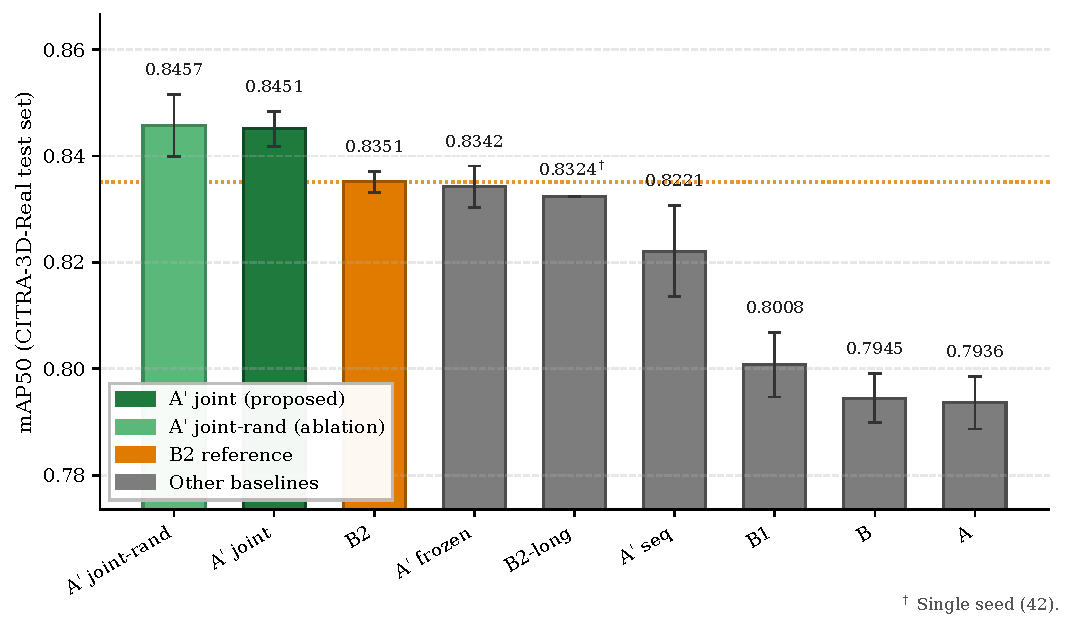
\includegraphics[width=\columnwidth]{fig6_comparison_bar}
%DIFDELCMD < %%%
\DIFdelendFL \DIFaddbeginFL 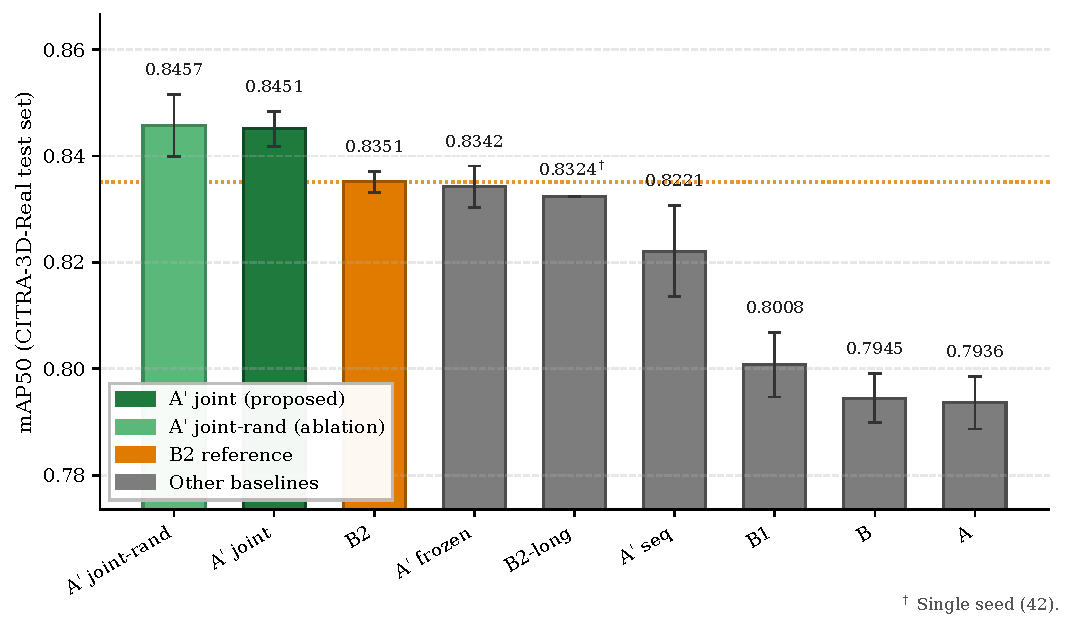
\includegraphics[width=0.80\columnwidth]{fig6_comparison_bar}
\DIFaddendFL \caption{mAP50 (top) and mAP50-95 (bottom) on the CITRA-3D-Real test set for all
experiment arms (mean over 3 seeds; error bars are one standard deviation). The
domain-adapted synthetic arms (A$'$ joint, A$'$ joint-rand) exceed the COCO
baseline (B2, dotted line), while naive InaTechShips pre-training (A, B) and
random initialisation (B1) fall below it. The volume-matched control B2-long (real images oversampled $13\times$, three seeds) coincides with B2 in mAP50, isolating the synthetic-diversity effect as the source of A$'$ joint's gain over B2.}
\label{fig:comparison}
\end{figure}

\begin{figure}[!t]
\centering
\DIFdelbeginFL %DIFDELCMD < 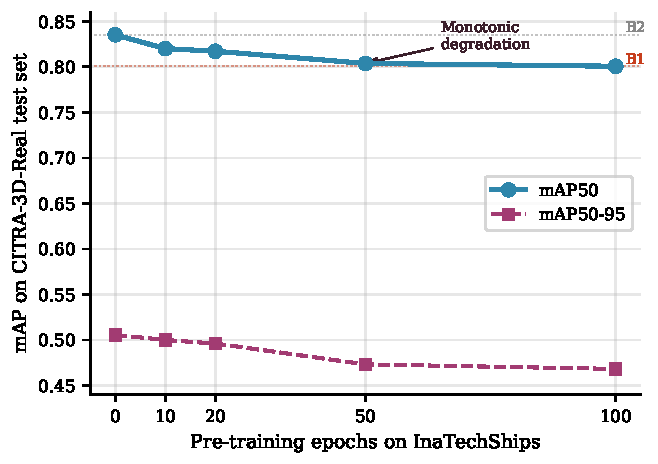
\includegraphics[width=\columnwidth]{fig5_ablation_curve}
%DIFDELCMD < %%%
\DIFdelendFL \DIFaddbeginFL 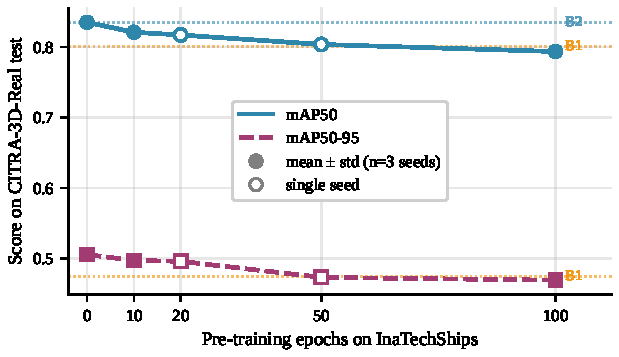
\includegraphics[width=\columnwidth]{fig4_ablation_curve}
\DIFaddendFL \caption{Downstream performance versus pre-training duration on the curated
public subset\DIFdelbeginFL \DIFdelFL{(diagnostic, seed 42)}\DIFdelendFL . Both mAP50 and mAP50-95 degrade monotonically with exposure,
approaching the random-initialisation level (B1); the COCO baseline (B2) is \DIFdelbeginFL \DIFdelFL{shown for reference}\DIFdelendFL \DIFaddbeginFL \DIFaddFL{the
0-epoch point. Filled markers with error bars: mean $\pm$ 1 std over 3 seeds
(0, 10, and 100 epochs); open markers: single seed (20 and 50)}\DIFaddendFL .}
\label{fig:epochs}
\end{figure}

\subsection{In-place composition and training regime}
\label{subsec:inplace}
Adapting the public crops to the operational domain reverses the picture, but the training regime is decisive. Sequential pre-training on synthetic data (A$'$ seq.) still degrades performance ($-1.31$ \DIFdelbegin \DIFdel{), and freezing }\DIFdelend \DIFaddbegin \DIFadd{on average, below the baseline in all three seeds, though not significant at $n{=}3$, $p=0.14$); extending the synthetic stage beyond 100 epochs is counter-indicated by the monotonic degradation in Fig.~\ref{fig:epochs}. Freezing }\DIFaddend the backbone during that phase is roughly neutral ($-0.09$)\DIFdelbegin \DIFdel{; only }\DIFdelend \DIFaddbegin \DIFadd{. Only }\DIFaddend \emph{balanced joint training} (A$'$ joint), which presents real and synthetic images together in a single run, yields a gain: $+1.00$ point in mAP50\DIFdelbegin \DIFdel{(non-overlapping mean\,$\pm$\,std ranges across seeds)}\DIFdelend \DIFaddbegin \DIFadd{, exceeding B2 in every seed ($p=0.024$; mAP50-95 $+1.50$, $p<0.001$), }\DIFaddend and Recall from $0.783$ to $0.805$ ($+2.2$ points\DIFaddbegin \DIFadd{, $p=0.013$}\DIFaddend ) without loss of Precision. 
A volume-matched control that oversamples the real images $13\times$ without synthetic data (B2-long, Table~\ref{tab:main}) matches the COCO baseline to within $0.0001$ in mAP50, so the $+1.00$-point mAP50 gain is attributable to synthetic diversity and the joint regime, not to training volume. The decomposition is metric-dependent: volume accounts for none of the mAP50 gain, about 30\% of the mAP50-95 gain, and most of the Recall gain (B2-long alone reaches Recall 0.796), consistent with additional real positives aiding recall while synthetic appearance diversity drives the precision-weighted improvements.

Stratifying by object size (Table~\ref{tab:size}) shows that the joint regime
improves \DIFdelbegin \DIFdel{all size categories, with the most relevant gain in small-object recall
}\DIFdelend \DIFaddbegin \DIFadd{every size category in all three seeds; the improvements are significant
for medium and large objects ($p<0.05$), while the largest point estimates occur
for small objects }\DIFaddend ($\text{AR}_\text{small}$ \DIFdelbegin \DIFdel{$0.385\!\rightarrow\!0.400$), which matters }\DIFdelend \DIFaddbegin \DIFadd{$0.390\!\rightarrow\!0.411$, $+2.1$
points, although not significant at $n{=}3$, $p=0.13$)---relevant }\DIFaddend because
71.6\% of operational vessels are small. This is consistent with the
interpretation that the synthetic vessel diversity helps the model recognise
appearances under-represented in the limited real set.

\begin{table}[!t]
\DIFdelbeginFL %DIFDELCMD < \renewcommand{\arraystretch}{1.15}
%DIFDELCMD < %%%
\DIFdelendFL \DIFaddbeginFL \renewcommand{\arraystretch}{1.05}
\DIFaddendFL \caption{AP and AR by object size (COCO \DIFdelbeginFL \DIFdelFL{convention}\DIFdelendFL \DIFaddbeginFL \DIFaddFL{thresholds applied in native image
pixels, $1920\times1080$}\DIFaddendFL ; mean $\pm$ std, 3 seeds).}
\label{tab:size}
\centering
\footnotesize
\DIFdelbeginFL %DIFDELCMD < \setlength{\tabcolsep}{6pt}
%DIFDELCMD < %%%
\DIFdelendFL \DIFaddbeginFL \setlength{\tabcolsep}{5pt}
\DIFaddendFL \begin{tabular}{@{}lcc@{}}
\toprule
Metric & B2 (COCO) & A$'$ joint \\
\midrule
$\text{AP}_\text{small}$  & \DIFdelbeginFL \DIFdelFL{$0.255 \pm 0.002$ }\DIFdelendFL \DIFaddbeginFL \DIFaddFL{$0.250 \pm 0.003$ }\DIFaddendFL & \DIFdelbeginFL \DIFdelFL{$0.262 \pm 0.011$ }\DIFdelendFL \DIFaddbeginFL \DIFaddFL{$0.271 \pm 0.005$ }\DIFaddendFL \\
$\text{AP}_\text{medium}$ & \DIFdelbeginFL \DIFdelFL{$0.571 \pm 0.002$ }\DIFdelendFL \DIFaddbeginFL \DIFaddFL{$0.569 \pm 0.003$ }\DIFaddendFL & \DIFdelbeginFL \DIFdelFL{$0.576 \pm 0.008$ }\DIFdelendFL \DIFaddbeginFL \DIFaddFL{$0.580 \pm 0.004$ }\DIFaddendFL \\
$\text{AP}_\text{large}$  & \DIFdelbeginFL \DIFdelFL{$0.679 \pm 0.001$ }\DIFdelendFL \DIFaddbeginFL \DIFaddFL{$0.686 \pm 0.004$ }\DIFaddendFL & \DIFdelbeginFL \DIFdelFL{$0.691 \pm 0.010$ }\DIFdelendFL \DIFaddbeginFL \DIFaddFL{$0.699 \pm 0.004$ }\DIFaddendFL \\
$\text{AR}_\text{small}$  & \DIFdelbeginFL \DIFdelFL{$0.385 \pm 0.007$ }\DIFdelendFL \DIFaddbeginFL \DIFaddFL{$0.390 \pm 0.011$ }\DIFaddendFL & \DIFdelbeginFL \DIFdelFL{$0.400 \pm 0.011$ }\DIFdelendFL \DIFaddbeginFL \DIFaddFL{$0.411 \pm 0.004$ }\DIFaddendFL \\
$\text{AR}_\text{medium}$ & \DIFdelbeginFL \DIFdelFL{$0.647 \pm 0.004$ }\DIFdelendFL \DIFaddbeginFL \DIFaddFL{$0.649 \pm 0.002$ }\DIFaddendFL & \DIFdelbeginFL \DIFdelFL{$0.655 \pm 0.004$ }\DIFdelendFL \DIFaddbeginFL \DIFaddFL{$0.658 \pm 0.005$ }\DIFaddendFL \\
$\text{AR}_\text{large}$  & \DIFdelbeginFL \DIFdelFL{$0.751 \pm 0.003$ }\DIFdelendFL \DIFaddbeginFL \DIFaddFL{$0.756 \pm 0.003$ }\DIFaddendFL & \DIFdelbeginFL \DIFdelFL{$0.759 \pm 0.010$ }\DIFdelendFL \DIFaddbeginFL \DIFaddFL{$0.767 \pm 0.002$ }\DIFaddendFL \\
\bottomrule
\end{tabular}
\end{table}

Finally, A$'$ joint-rand---which places synthetic crops at random sea positions
rather than at real-vessel positions---reaches statistically comparable accuracy
to A$'$ joint, showing that exact spatial anchoring is not the driver: within the
balanced joint regime the gain comes from crop diversity, scale/density
alignment, and the training regime itself. \DIFdelbegin \DIFdel{In-place anchoring nonetheless remains
a useful default, since it guarantees plausible placement by construction and avoids the need to model }\DIFdelend \DIFaddbegin \DIFadd{Out of domain the random variant is in
fact consistently better ($+1.91$ pp over A$'$~joint on SMD, all three seeds,
$p=0.005$; Table~\ref{tab:smd_results}). We therefore recommend in-place
anchoring when auditability and }\DIFaddend the \DIFdelbegin \DIFdel{sea region explicitly}\DIFdelend \DIFaddbegin \DIFadd{absence of placement heuristics matter---every
synthetic position inherits a real observation, with no sea-region model or
inpainting required---and sea-aware random placement when cross-domain
generalisation is the priority}\DIFaddend .

\subsection{Zero-shot cross-domain generalisation}
\label{subsec:zeroshot}

To test whether these effects are properties of the approach rather than of the
CITRA-3D-Real test set, we evaluate all models, without any fine-tuning, on an
independent dataset: the visible on-shore subset of the Singapore Maritime
Dataset (SMD) \cite{prasad2017video}. We keep only fixed-camera on-shore footage,
collapse annotations to the single \emph{vessel} class, re-split by source video
to preclude leakage, and temporally subsample frames, yielding 914 images from 36
videos. Table~\ref{tab:smd_results} shows that both directional effects reproduce on this
unseen domain: the synthetic arms exceed the COCO baseline while both InaTechShips
arms fall below it, and random initialisation is worst. As expected under a domain
shift, absolute accuracy drops and seed-to-seed variance grows, so \DIFdelbegin \DIFdel{the two
synthetic arms are statistically comparable to each
other and only clearly
}\DIFdelend \DIFaddbegin \DIFadd{each
synthetic arm is }\DIFaddend separated from B2 \DIFdelbegin \DIFdel{in mean; nevertheless, }\DIFdelend \DIFaddbegin \DIFadd{only in mean (A$'$~joint vs.\ B2, $p=0.41$),
while between the synthetic arms the random-placement variant consistently
exceeds the anchored one ($+1.91$ pp, $p=0.005$; Sec.~\ref{subsec:inplace});
}\DIFaddend the ordering---domain-adapted synthetic $>$ COCO $>$ naive public---is
preserved. \DIFaddbegin \DIFadd{A$'$~seq., which degrades in-domain, is statistically
indistinguishable from B2 out of domain ($0.6026\pm0.0373$, the largest seed
variance in the table), indicating that the damage of the sequential regime is
specific to in-domain fine-tuning rather than a general corruption of
features. }\DIFaddend This indicates that neither the negative
transfer of public pre-training nor the benefit of domain-adapted composition is
an artefact of the operational test set.

Volume control under domain shift. The volume-matched control B2-long, which equalled the COCO baseline in-domain, falls \DIFdelbegin \DIFdel{$1.1$ }\DIFdelend \DIFaddbegin \DIFadd{$1.6$ }\DIFaddend pp below B2 on SMD (Table~\ref{tab:smd_results}). Real-image oversampling thus not only fails to provide the gain that synthetic composition delivers, but mildly hurts out-of-domain generalisation, consistent with mild overfitting to CITRA-3D-Real's distribution. The gap between A' joint and B2-long widens from $+1.00$ pp on CITRA to \DIFdelbegin \DIFdel{$+2.47$ }\DIFdelend \DIFaddbegin \DIFadd{$+2.96$ }\DIFaddend pp on SMD, indicating that the contribution of synthetic diversity is relatively more important under domain shift than within-domain.

\begin{table*}[t]
\caption{Zero-shot cross-domain results on the SMD on-shore subset (914 images, 36 videos; no fine-tuning on SMD). Mean $\pm$ std over 3 seeds; $\Delta$ versus B2 in points.}
\label{tab:smd_results}
\centering
\begin{tabular}{lccr}
\toprule
Method & mAP50 & mAP50-95 & $\Delta$ \\
\midrule
A' joint-rand (ablation)  & 0.6193 $\pm$ 0.0030 & 0.3082 $\pm$ 0.0040 & $+$3.25 \\
A' frozen                 & 0.6080 $\pm$ 0.0018 & 0.2982 $\pm$ 0.0056 & $+$2.12 \\
A' \DIFaddbeginFL \DIFaddFL{seq.                   }& \DIFaddFL{0.6026 $\pm$ 0.0373 }& \DIFaddFL{0.2978 $\pm$ 0.0159 }& \DIFaddFL{$+$1.58 }\\
\DIFaddFL{A' }\DIFaddendFL joint (proposed)       & 0.6002 $\pm$ 0.0043 & 0.2926 $\pm$ 0.0041 & $+$1.34 \\
B2 (COCO, reference)      & 0.5868 $\pm$ 0.0160 & 0.2900 $\pm$ 0.0064 & ref \\
B2-long (volume control)  & \DIFdelbeginFL \DIFdelFL{0.5755 }\DIFdelendFL \DIFaddbeginFL \DIFaddFL{0.5706 }\DIFaddendFL $\pm$ \DIFdelbeginFL \DIFdelFL{0.0131 }\DIFdelendFL \DIFaddbeginFL \DIFaddFL{0.0063 }\DIFaddendFL & \DIFdelbeginFL \DIFdelFL{0.2879 }\DIFdelendFL \DIFaddbeginFL \DIFaddFL{0.2833 }\DIFaddendFL $\pm$ \DIFdelbeginFL \DIFdelFL{0.0089 }\DIFdelendFL \DIFaddbeginFL \DIFaddFL{0.0048 }\DIFaddendFL & $-$\DIFdelbeginFL \DIFdelFL{1.13 }\DIFdelendFL \DIFaddbeginFL \DIFaddFL{1.62 }\DIFaddendFL \\
A (InaTech curated)       & 0.5661 $\pm$ 0.0241 & 0.2805 $\pm$ 0.0125 & $-$2.07 \\
B (InaTech random)        & 0.5508 $\pm$ 0.0215 & 0.2700 $\pm$ 0.0115 & $-$3.60 \\
B1 (random init)          & 0.4924 $\pm$ 0.0128 & 0.2337 $\pm$ 0.0037 & $-$9.44 \\
\bottomrule
\end{tabular}
\end{table*}

\section{Discussion}
\textbf{Localising the cause of the negative transfer.} Arms A, A$'$ seq, and
A$'$ joint draw their vessel appearance from the same public source and differ
only in how that content is presented to the network, which turns the comparison
into a controlled dissection. Direct pre-training on the unmodified public images
(A, $-4.15$) shares the target's semantic class but not its object-level
structure: vessels are large, isolated, and photographed at close range.
Realigning the same crops to the target's scale, density, and capture context as
an intermediate sequential stage (A$'$ seq, $-1.31$) roughly halves the
degradation. Because the source vessel content is held fixed between A and
A$'$ seq, this improvement is attributable to structural rather than semantic
factors. The dominant structural difference is scale---operational vessels are
about \DIFdelbegin \DIFdel{$500\times$ }\DIFdelend \DIFaddbegin \DIFadd{$400\times$ }\DIFaddend smaller in normalised area (Table~\ref{tab:gap},
Fig.~\ref{fig:scale})---so we attribute the bulk of the effect to object-scale
mismatch, while noting that our composites align scale, density, and context
jointly and therefore do not isolate their individual contributions.

\textbf{Why the joint regime is necessary.} Structural realignment alone does not
suffice: A$'$ seq stays below the COCO baseline because sequential pre-training
still specialises---and partially overwrites---the generic COCO features before
the target is seen, consistent with the monotonic degradation of
Fig.~\ref{fig:epochs} and a forgetting-like mechanism
\cite{mccloskey1989catastrophic}. Only balanced joint training (A$'$ joint,
$+1.00$) presents real and structurally-aligned synthetic images together,
exploiting the added vessel diversity without discarding the COCO prior. The
progression $-4.15 \rightarrow -1.31 \rightarrow +1.00$ therefore separates two
factors: structural alignment governs how much the source \emph{can} help, and
the training regime governs whether that help is \emph{realised} (Fig.~\ref{fig:mechanism}); freezing the backbone during sequential pre-training (A$'$ frozen, $-0.09$) protects the COCO
prior but forgoes most of the benefit.

\begin{figure}[!t]
\centering
\DIFdelbeginFL %DIFDELCMD < 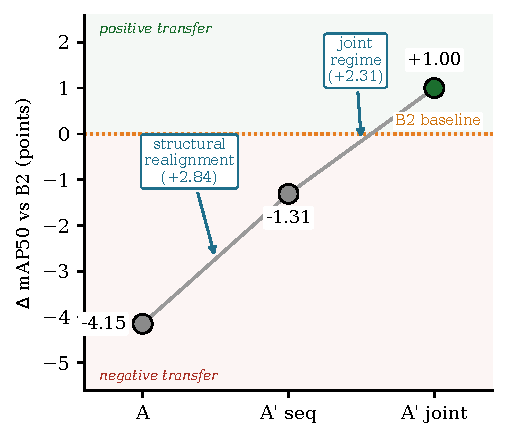
\includegraphics[width=\columnwidth]{fig_mechanism}
%DIFDELCMD < %%%
\DIFdelendFL \DIFaddbeginFL 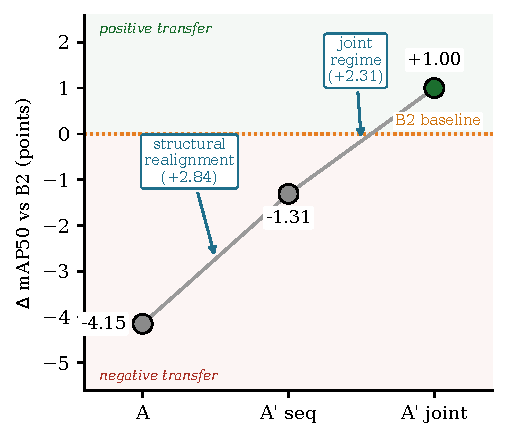
\includegraphics[width=0.84\columnwidth]{fig_mechanism}
\DIFaddendFL \caption{Mechanism decomposition. Holding the source vessel content fixed,
structural realignment (A\,$\rightarrow$\,A$'$ seq) and the balanced joint regime
(A$'$ seq\,$\rightarrow$\,A$'$ joint) each contribute a separable gain, moving the
outcome from strong negative transfer to a positive gain over the COCO baseline.}
\label{fig:mechanism}
\end{figure}

\textbf{Operational relevance.} In maritime surveillance, where missed detections
are costlier than false alarms, the Recall gain at no Precision \DIFdelbegin \DIFdel{cost---largest }\DIFdelend \DIFaddbegin \DIFadd{cost---with the
largest point estimate }\DIFaddend in the small-object regime (Table~\ref{tab:size})---is the
operationally meaningful outcome.

\textbf{Limitations.} Our composites vary scale, density, and context together,
so we identify structural mismatch as the driver of the negative transfer but do
not isolate the contribution of each axis; a factorial design that perturbs one
axis at a time is left to future work. The primary evaluation also uses a single
operational dataset---the zero-shot probe on SMD indicates the effects persist on
an independent domain---and a single detector architecture; broader validation
remains future work.

\section{Conclusion}
We showed that naive use of a large public ship dataset for pre-training causes
negative transfer in operational maritime vessel detection, driven by a structural
domain gap that \DIFaddbegin \DIFadd{global }\DIFaddend visual-similarity curation does not address and that
worsens monotonically with pre-training exposure. In-place synthetic composition
combined with balanced joint training converts this into a modest but consistent
improvement in mAP50 and \DIFdelbegin \DIFdel{small-object Recall }\DIFdelend \DIFaddbegin \DIFadd{Recall across all object sizes}\DIFaddend , and a controlled ablation shows that
the gain is attributable to crop diversity, scale/density alignment, and the
training regime rather than to exact spatial anchoring. A zero-shot evaluation on
an independent dataset confirms both directional effects on an unseen domain.
Future work includes multi-class detection, alternative detector architectures, a factorial decomposition of the structural gap (scale, density, context) via single-axis interventions, and the optimal ratio of real to synthetic images in joint training.

\iffinal
\section*{Acknowledgment}
% Add funding and acknowledgments only in the camera-ready version.
\fi

\bibliographystyle{IEEEtran}
\bibliography{references}

\end{document}
